\subsection{Progettazione di dettaglio e codifica}
Questa fase comincia in seguito a quella precedente e termina con la \textit{Revisione di Qualifica}, ovvero dal 08-03-2021 al 02-04-2021. Durante questa fase verranno implementate buona parte delle componenti della web app e verranno anche aggiunte funzionalità alle componenti già sviluppate in precedenza.
Di seguito è riportato il dettaglio di ogni incremento.

\subsubsection{Incremento III}
\textit{dal 08-03-2021 al 13-03-2021}\\
L'incremento III prevede la progettazione di dettaglio e codifica delle componenti software. Si prevede di svolgere quanto segue:
\begin{itemize}
\item Implementazione di un componente per applicare una riduzione dimensionale ai dati;
\item Aggiunta di alcuni controlli per la configurazione dei parametri relativi ai diversi algoritmi di riduzione dimensionale disponibili.
\end{itemize}
\textbf{Attività}
\begin{itemize}
\item \textbf{Stesura:} eventuali correzioni ai documenti ed inizio stesura dell'allegato tecnico con scelta dei design patterns;
\item \textbf{Verifica documenti}
\item \textbf{Progettazione:} progettazione del componente per la riduzione dimensionale;
\item \textbf{Codifica:} codifica del componente per la riduzione dimensionale con relativa parametrizzazione;
\item \textbf{Verifica software:} verifica sulle funzionalità software aggiunte.
\end{itemize}
\subsubsection{Incremento IV}
\textit{dal 13-03-2021 al 17-03-2021}\\
L'incremento IV prevede la progettazione di dettaglio e codifica delle componenti software. Si prevede di svolgere quanto segue:
\begin{itemize}
\item Implementazione della visualizzazione Heat Map;
\item Aggiunta di alcuni controlli per la configurazione dei parametri relativi alla visualizzazione precedentemente implementata.
\end{itemize}
\textbf{Attività}
\begin{itemize}
\item \textbf{Stesura:} incremento della documentazione da allegare al prodotto;
\item \textbf{Verifica documenti}
\item \textbf{Progettazione:} progettazione del componente per la visualizzazione Heat Map;
\item \textbf{Codifica:} codifica del componente per la visualizzazione con relativa parametrizzazione;
\item \textbf{Verifica software:} verifica sulle funzionalità software aggiunte.
\end{itemize}

\subsubsection{Incremento V}
\textit{dal 17-03-2021 al 21-03-2021}\\
L'incremento V prevede la progettazione di dettaglio e codifica delle componenti software. Si prevede di svolgere quanto segue:
\begin{itemize}
\item Implementazione della visualizzazione Force Field;
\item Aggiunta di alcuni controlli per la configurazione dei parametri relativi alla visualizzazione precedentemente implementata.
\end{itemize}
\textbf{Attività}
\begin{itemize}
\item \textbf{Stesura:} incremento della documentazione da allegare al prodotto e inizio del manuale utente e del manuale manutentore;
\item \textbf{Verifica documenti}
\item \textbf{Progettazione:} progettazione del componente per la visualizzazione Force Field;
\item \textbf{Codifica:} codifica del componente per la visualizzazione con relativa parametrizzazione;
\item \textbf{Verifica software:} verifica sulle funzionalità software aggiunte.
\end{itemize}

\subsubsection{Incremento VI}
\textit{dal 21-03-2021 al 26-03-2021}\\
L'incremento V prevede la progettazione di dettaglio e codifica delle componenti software. Si prevede di svolgere quanto segue:
\begin{itemize}
\item Implementazione della visualizzazione Proiezione Lineare Multi Asse;
\item Aggiunta di alcuni controlli per la configurazione dei parametri relativi alla visualizzazione precedentemente implementata.
\end{itemize}
\textbf{Attività}
\begin{itemize}
\item \textbf{Stesura:} incremento della documentazione da allegare al prodotto ;
\item \textbf{Verifica documenti}
\item \textbf{Progettazione:} progettazione del componente per la visualizzazione Proiezione Lineare Multi Asse;
\item \textbf{Codifica:} codifica del componente per la visualizzazione con relativa parametrizzazione;
\item \textbf{Verifica software:} verifica sulle funzionalità software aggiunte.
\end{itemize}

\subsubsection{Incremento VII}
\textit{dal 26-03-2021 al 2-04-2021}\\
L'incremento V prevede la progettazione di dettaglio e codifica delle componenti software. Si prevede di svolgere quanto segue:
\begin{itemize}
\item Implementazione di un database;
\item Sviluppo di un componente per la scelta e il caricamento di un dataset contenuto nel database.
\end{itemize}
\textbf{Attività}
\begin{itemize}
\item \textbf{Stesura:} incremento e conclusione della documentazione da allegare al prodotto ;
\item \textbf{Verifica documenti}
\item \textbf{Progettazione:} progettazione del database e del componente per la scelta e il caricamento del dataset;
\item \textbf{Creazione struttura database:} stesura della struttura del database;
\item \textbf{Codifica:} codifica del componente per la scelta e il caricamento del dataset;
\item \textbf{Verifica software:} verifica sulle funzionalità software aggiunte.
\end{itemize}

\begin{landscape}

\begin{figure}[h]
 	\centering
	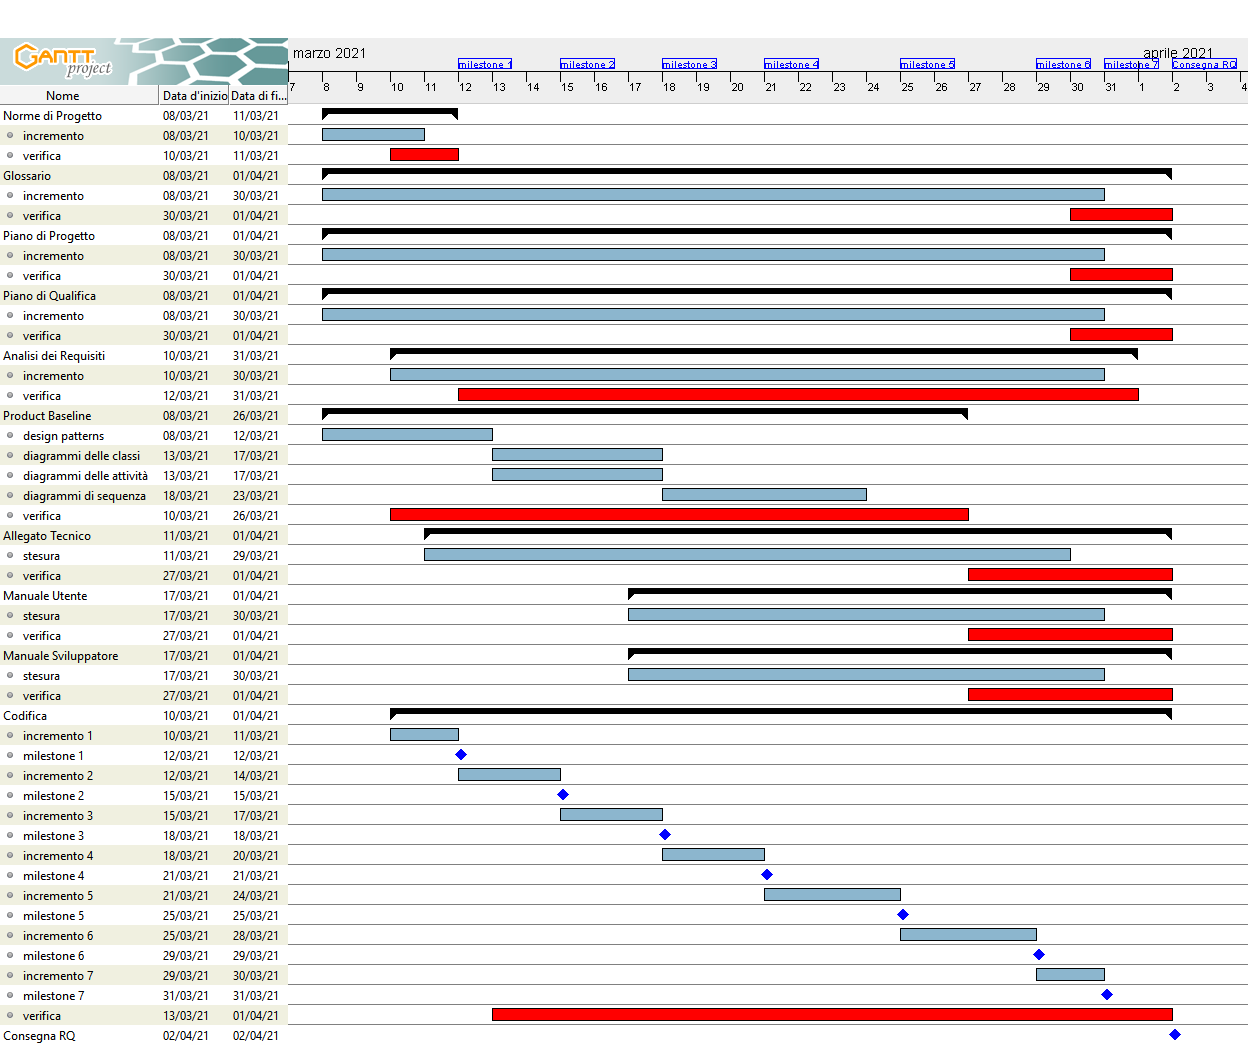
\includegraphics[width=\linewidth]{Images/GanttPianificazioneProgettazioneDettaglioCodifica.png}
	\caption{Diagramma di Gantt dell'attività di Progettazione di dettaglio e Codifica}
\end{figure}

\end{landscape}